\documentclass[thesis.tex]{subfiles}

\ifSubfilesClassLoaded{
  \externaldocument{thesis}
  \setcounter{chapter}{2}
}{}

\begin{document}
\chapter{Fixpoints for representation predicates} \label{ch:fixpoints}
In this chapter we show how non-structurally recursive representation predicates can be defined using least fixpoints. In \cref{sec:fixproblem} we explain why it is hard to define non-structurally recursive predicates and generally explain the approach that is taken. Next, in \cref{sec:fixIris} we show the way least fixpoints are defined in Iris. Lastly, in \cref{sec:monoproofsearch} we explain the improvements we made to the approach of Iris in order for the process to be automated.

\section{Problem statement} \label{sec:fixproblem}
In order to define a recursive predicate we have to prove it actually exists. One way of defining recursive predicates is by structural recursion. Thus, every recursive call in the predicate has to be on a structurally smaller part of the arguments.

The candidate argument for structural recursion in $\isMLL$ would be the list of values used to represent the MLL. However, this does not work given the second case of the recursion.
\begin{align*}
  \isMLL\,\hd\,\vect{\val} = \cdots \lor (\Exists \loc, \val', \tl. \hd = \Some l * l \fmapsto (\val', \True, \tl) * \isMLL\, \tl\, \vect{\val}) \lor \cdots
\end{align*}
Here the list of values is passed straight onto the recursive call to $\isMLL$. Thus, it is not structurally recursive.

We need another approach to define non-structurally recursive predicates such as these. Iris has several approaches to fix this problem, as is discussed in \cref{ch:relatedwork}. The approach we use as the basis of eiInd is the least fixpoint, inspired by the Knaster-Tarski fixpoint theorem \cite*{tarskiLatticetheoreticalFixpointTheorem1955}. Given a monotone function on predicates, there exists a least fixpoint of this function. We can now choose a function such that the fixpoint corresponds to the recursive predicate we wanted to design. This procedure is explained thoroughly in the next section, \cref{sec:fixIris}.

\section{Least fixpoint in Iris} \label{sec:fixIris}
To define a least fixpoint in Iris the first step is to have a monotone function.
\begin{definition}{Monotone function}{monofunc}
  Function $\hopred\colon (A \to \iProp) \to  A \to \iProp$ is monotone when for any $\pred, \predB\colon A \to \iProp$, it holds that
  \[ \always(\All \varB. \pred\,\varB \wand \predB\,\varB) \proves \All \var. \hopred\,\pred\,\var \wand \hopred\,\predB\,\var\]
  In other words, $\hopred$ is monotone in its first argument.
\end{definition}
This definition of monotone follows the definition of monotone in other fields with one exception. The assumption has an additional restriction, it has to be persistent. The persistence is necessary since $\hopred$ could use its monotone argument multiple times.
\begin{example}{}{treemono}
  Take the following function.
  \begin{align*}
    \hopred\, \pred\, \val \eqdef{} & (\val = \None) \lor{}                                                                                                                                  \\
                                    & (\Exists \loc_1,\loc_2,\val_1,\val_2. \val = \Some (\loc_1, \loc_2) * \loc_1 \fmapsto \val_1 * \loc_2 \fmapsto \val_2 * \pred\,\val_1 * \pred\,\val_2)
  \end{align*}
  This is the function for binary trees. The value $\val$ is either empty, and we have an empty tree. Or $\val$ contains two locations, for the two branches of the tree. Each location points to a value and $\pred$ is holds for both of these values. The fixpoint, as is discussed in \cref{thm:leastfixpoint}, of this function holds for a value containing a binary tree. However, before we can take the fixpoint we have to prove it is monotone.
  \[\always(\All \valB. \pred\,\valB \wand \predB\,\valB) \proves \All \val. \hopred\, \pred\, \val \wand \hopred\, \predB\, \val\]
  \begin{proof}
    We start by introducing $\val$ and the wand.
    \begin{align*}
      \always(\All \valB. \pred\,\valB \wand \predB\,\valB) * \hopred\, \pred\, \val \proves \hopred\, \predB\, \val
    \end{align*}
    We now unfold the definition of $\hopred$ and eliminate and introduce the disjunction, resulting in two statements to prove.
    \[\always(\All \valB. \pred\,\valB \wand \predB\,\valB) * \val = \None \proves \val = \None\]
    \begin{align*}
       & \always(\All \valB. \pred\,\valB \wand \predB\,\valB) * \left(\Exists \loc_1,\loc_2,\val_1,\val_2.
      \begin{array}{l}
        \val = \Some (\loc_1, \loc_2) * \loc_1 \fmapsto \val_1 *{} \\
        \loc_2 \fmapsto \val_2 * \pred\,\val_1 * \pred\,\val_2
      \end{array}\right)
      \proves                                                                                               \\
       & \left(\Exists \loc_1,\loc_2,\val_1,\val_2.
      \begin{array}{l}
        \val = \Some (\loc_1, \loc_2) * \loc_1 \fmapsto \val_1 *{} \\
        \loc_2 \fmapsto \val_2 * \predB\,\val_1 * \predB\,\val_2
      \end{array}\right)
    \end{align*}
    The first statement holds directly. For the second statement we eliminate the existentials in the assumption and use the created variables to introduce the existentials in the conclusion.
    \begin{align*}
       & \always(\All \valB. \pred\,\valB \wand \predB\,\valB) *
      \begin{array}{l}
        \val = \Some (\loc_1, \loc_2) *{}                   \\
        \loc_1 \fmapsto \val_1 * \loc_2 \fmapsto \val_2 *{} \\
        \pred\,\val_1 * \pred\,\val_2
      \end{array}
      \proves
      \begin{array}{l}
        \val = \Some (\loc_1, \loc_2) *{}                   \\
        \loc_1 \fmapsto \val_1 * \loc_2 \fmapsto \val_2 *{} \\
        \predB\,\val_1 * \predB\,\val_2
      \end{array}
    \end{align*}
    Any sub propositions that occur both on the left and right-hand side are canceled out using \ruleref{sep-mono}.
    \begin{align*}
       & \always(\All \valB. \pred\,\valB \wand \predB\,\valB) * \pred\,\val_1 * \pred\,\val_2
      \proves \predB\,\val_1 * \predB\,\val_2
    \end{align*}
    We want to split the conclusion and premise in two, such that we get the following statements, with $i\in\{1,2\}$.
    \begin{align*}
       & \always(\All \valB. \pred\,\valB \wand \predB\,\valB) * \pred\,\val_i
      \proves \predB\,\val_i
    \end{align*}
    To achieve this split, we duplicate the persistent premise and then split using \ruleref{sep-mono} again. Both these statements hold trivially.
  \end{proof}
  \noindent In the previous proof it was essential that the premise of monotonicity is persistent. This occurs any time we have a data structure with more than one branch.
\end{example}
Now that we have a definition of a function, we can prove that a least fixpoint of a monotone function always exists.
\begin{theorem}{Least fixpoint}{leastfixpoint}
  Given a monotone function $\hopred\colon (A \to \iProp) \to  A \to \iProp$, called the \emph{pre fixpoint function}, there exists a least fixpoint $\lfp\hopred\colon  A \to \iProp$ such that
  \begin{enumerate}
    \item The fixpoint equality holds
          \[ \lfp\hopred\, \var \provesIff \hopred\, (\lfp\hopred)\, \var \]
    \item The iteration property holds
          \[ \always \All \varB. \hopred\, \pred\, \varB \wand \pred\, \varB \proves \All \var. \lfp\hopred\, \var \wand \pred\, \var \]
  \end{enumerate}
\end{theorem}
\begin{proof}
  Given a monotone function $\hopred\colon (A \to \iProp) \to  A \to \iProp$ we define $\lfp\hopred$ as
  \[ \lfp\hopred\, \var \eqdef \All \pred. \always(\All \varB. \hopred\, \pred\, \varB \wand \pred\, \varB) \wand \pred \, \var \]
  We now prove the two properties of the least fixpoint
  \begin{enumerate}
    \item The right to left direction follows from monotonicity of $\hopred$. The left to right direction follows easily from monotonicity of $\hopred$ and the right to left direction.
    \item This follows directly from unfolding the definition of $\lfp\hopred$. \qedhere
  \end{enumerate}
\end{proof}
\noindent The first property of \cref{thm:leastfixpoint}, fixpoint equality, defines that the least fixpoint is a fixpoint. The second property of \cref{thm:leastfixpoint}, iteration, ensures that this fixpoint is the least of the possible fixpoints. The iteration property is a simpler version of the induction principle. The induction hypothesis during iteration is simpler. It only ensures that $\pred$ holds under $\hopred$. Full induction requires that we also know that the fixpoint holds under $\hopred$ in the induction hypothesis.
\begin{lemma}{Induction principle}{fixind}
  Given a monotone predicate $\hopred\colon (\sigax \to \iProp) \to (\sigax \to \iProp)$, it holds that
  \[\always(\All\var.\hopred\,(\Lam\varB. \pred\,\varB \land \lfp\hopred\,\varB)\,\var \wand \pred\,\var) \wand \All\var. \lfp\hopred\,\var \wand \pred\,\var\]
\end{lemma}
\begin{proof}
  The induction principle for a $\predB$ holds by the iteration property with $\pred \var = \predB\, \var \land \lfp\hopred\, \var$
\end{proof}
This lemma follows from monotonicity and the least fixpoint properties.

We can now use the above steps to define $\isMLL$
\begin{example}{Iris least fixpoint of $\isMLL$}{irisisMLL}
  We want to create a least fixpoint such that it has the following inductive property.
  \begin{align*}
    \isMLL\, \hd\, \vect{\val} & = \isMLLRecDef
  \end{align*}
  The first step is creating the pre fixpoint function. We do this by adding an argument to $\isMLL$ transforming it into a function. We then substitute any recursive calls to $\isMLL$ with this argument.
  \begin{align*}
    \isMLL_\hopred\, \pred\, \hd\, \vect{v} & \eqdef
    \isMLLFDef
  \end{align*}
  This has created a function, $\isMLL_\hopred$. The function applies the predicate, $\pred$, on the tail of any possible MLL, while ensuring the head is part of an MLL. Next, we want to prove that $\isMLL_\hopred$ is monotone. However, $\isMLL_\hopred$ has the following type.
  \[\isMLL_\hopred\colon (\Val \to \List\ \Val \to \iProp) \to \Val \to \List\ \Val \to \iProp\]
  But, \cref{def:monofunc} only works for functions of type
  \[\hopred\colon (\sigax \to \iProp) \to \sigax \to \iProp\]
  This is solved by uncurrying $\isMLL_\hopred$
  \begin{align*}
    \isMLL'_\hopred\, \pred\, (\hd, \vect{\val}) \eqdef \isMLL_\hopred\, \pred\, \hd\, \vect{\val}
  \end{align*}
  The function $\isMLL'_\hopred$ now has the type
  \[\isMLL'_\hopred\colon (\Val \carprod \List\ \Val \to \iProp) \to  \Val \carprod \List\ \Val \to \iProp\]
  And we can prove $\isMLL_\hopred$ is monotone.
  \begin{align*}
              & \always(\All(\hd, \vect{\val}). \pred\,(\hd, \vect{\val}) \wand \predB\,(\hd, \vect{\val}))                              \\
    \proves{} & \All(\hd, \vect{\val}). \isMLL'_\hopred\, \pred\, (\hd, \vect{\val}) \wand \isMLL'_\hopred\, \predB\, (\hd, \vect{\val})
  \end{align*}
  \begin{proof}
    We use a similar proof as in \cref{ex:treemono}. It involves more steps as we have more branches, but the same ideas apply.
  \end{proof}
  Given that $\isMLL'_\hopred$ is monotone, we now know from \cref{thm:leastfixpoint} that the least fixpoint exists of $\isMLL'_\hopred$. By uncurrying we can create the final definition of $\isMLL$.
  \begin{align*}
    \isMLL\, \hd\, \vect{\val} \eqdef \lfp(\isMLL'_\hopred)\, (\hd, \vect{\val})
  \end{align*}
  This definition of $\isMLL$ has the inductive property as described in \cref{sec:represpreds}. That property is the fixpoint equality. After expanding any currying, we get the below induction principle for $\isMLL$ from \cref{lem:fixind}.
  \begin{align*}
     & \begin{array}{l}
         \always(\All\hd,\vect{\val}.\isMLL_\hopred\,(\Lam\hd',\vect{\val}'. \pred\,\hd'\,\vect{\val}' \land \isMLL\,\hd'\,\vect{\val}')\,\hd\,\vect{\val} \wand \pred\,\hd\,\vect{\val}) \\
         \wand \All\hd,\vect{\val}. \isMLL\,\hd\,\vect{\val} \wand \pred\,\hd\,\vect{\val}
       \end{array}
  \end{align*}
  The induction principle from \cref{sec:represpreds} is also derivable from \cref{lem:fixind}. The three cases of the induction principle follow from the disjunctions in $\isMLL_\hopred$.

\end{example}

\section{Syntactic monotone proof search}
\label{sec:monoproofsearch}%
As we discussed in \cref{ch:introduction}, the goal of this thesis is to show how to automate the definition of representation predicates from inductive definitions. The major hurdle in this process can be seen in \cref{ex:irisisMLL}, proving a function monotone. In this section we show how a monotonicity proof can be found by using syntactic proof search.

We base our strategy on the work by \Citeauthor{sozeauNewLookGeneralized2009} \cite{sozeauNewLookGeneralized2009}. They create a system for rewriting expressions in goals in Coq under generalized relations, instead of just equality. Many definitions are equal, but do them in separation logic instead of the logic of Coq. The proof search itself is not based on the generalized rewriting of \Citeauthor{sozeauNewLookGeneralized2009}.

We take the following strategy. We prove the monotonicity of all the connectives once. We now prove the monotonicity of the function by making use of the monotonicity of the connectives with which it is built.

\paragraph*{Monotone connectives}
We don't want to uncurry every connective when using that it is monotone, thus we take a different approach on what is monotone. For every connective we give a signature telling us how it is monotone. We show a few of these signatures below.

\begin{center}
  \begin{tabular}{lll}
    Connective & Type                           & Signature                                           \\
    \hline
    $*$        & $\Prop \to \Prop \to \Prop$    & $\wandrel \respect \wandrel \respect \wandrel$      \\
    $\lor$     & $\Prop \to \Prop \to \Prop$    & $\wandrel \respect \wandrel \respect \wandrel$      \\
    $\wand$    & $\Prop \to \Prop \to \Prop$    & $\flip\wandrel \respect \wandrel \respect \wandrel$ \\
    $\exists$  & $(\sigax \to \Prop) \to \Prop$ & $(\eqrel \respect \wandrel) \respect \wandrel$
  \end{tabular}
\end{center}
We make use of the Haskell prefix notation, $(\wand)$, to turn an infix operator into a prefix function. The signature of a connective defines the requirements for monotonicity a connective has. The signatures are based on building relations which we can apply on the connectives.
\begin{definition}{Relation in $\iProp$}{irel}
  A relation in separation logic on type $\sigax$ is defined as
  \[\Rel\ \sigax \eqdef \sigax \to \sigax \to \Prop\]
\end{definition}
The combinators used to build signatures now build relations.
\begin{definition}{Respectful relation}{respect}
  The respectful relation $\rel \respect \rel'\colon \Rel\ (\sigax\to\sigaxB)$ of two relations $\rel\colon\Rel\ \sigax$, $\rel'\colon\Rel\ \sigaxB$ is defined as
  \begin{align*}
    \rel \respect \rel' \eqdef \Lam \func, \funcB. \All \var,\varB. \rel\, \var\, \varB \wand \rel'\, (\func\, \var)\, (\funcB\, \varB)
  \end{align*}
\end{definition}
\begin{definition}{Flipped relation}{flip}
  The flipped relation $\flip\, \rel\colon\Rel\ \sigax$ of a relation $\rel\colon\Rel\ \sigax$ is defined as
  \[\flip\, \rel \eqdef \Lam \var, \varB. \rel\, \varB\, \var\]
\end{definition}
Given a signature we can define when a connective has a signature.
\begin{definition}{Proper element of a relation}{proper}
  Given a relation $\rel\colon\Rel\ \sigax$ and an element $\var\in\sigax$, $\var$ is a proper element of $\rel$ if $\rel\, \var\, \var$
\end{definition}
We define how a connective is monotone by the signature it is a proper element of. The proofs that the connectives are the proper elements of their signature are fairly trivial, but we will highlight the existential qualifier.

\quest{I want to expand the first two signatures, but I don't have anything interesting to say about it except for showing the expanded version}
% Both the separating conjunction and the disjunction have the same signature, when filling in the seperating conjunction we get the following statement
% \[ \All \prop, \prop'. (\prop \wand \prop') \wand \All \propB, \propB'. (\propB \wand \propB') \wand (\prop * \propB) \wand (\prop' * \propB') \]

We can unfold the definitions in the signature and fill in the existential quantification in order to get the following statement,
\[\All \pred, \predB. (\All \var, \varB. \var = \varB \wand \pred\, \var \wand \predB\, \varB) \wand (\Exists \var. \pred\, \var) \wand (\Exists \var. \predB\, \var) \]
This statement can be easily simplified by substituting $\varB$ for $\var$ in the first relation.
\[\All \pred, \predB. (\All \var. \pred\, \var \wand \predB\, \var) \wand (\Exists \var. \pred\, \var) \wand (\Exists \var. \predB\, \var) \]
We create a new combinator for signatures, the pointwise relation, to include the above simplification in signatures.
\begin{definition}{Pointwise relation}{pointwise}
  The pointwise relation $\point \rel$ is a special case of a respectful relation defined as
  \begin{align*}
    \point \rel \eqdef \Lam \func, \funcB. \All \var. \rel\, (\func\, \var)\, (\funcB\, \varB)
  \end{align*}
\end{definition}
The new signature for the existential quantification becomes
\[\point \wandrel \respect \wandrel\]

\paragraph*{Monotone functions}
To create a monotone function for the least fixpoint we need to be able to at least define \cref{def:monofunc} in terms of the proper element of a signature. We already have most the combinators needed, but we are missing a way to mark a relation as persistent.
\begin{definition}{Persistent relation}{persrel}
  The persistent relation $\persrel\rel\colon\Rel\ \sigax$ for a relation $\rel\colon\Rel\ \sigax$ is defined as
  \[\persrel\rel \eqdef \Lam\var,\varB. \always (\rel\,\var\,\varB)\]
\end{definition}
Thus we can create the following signature for \cref{def:monofunc}.
\[\persrel (\point \wandrel) \respect \point \wandrel\]
Filling in an $\hopred$ as the proper element get the following statement.
\[ \always(\All \varB. \pred\,\varB \wand \predB\,\varB) \wand \All \var. \hopred\,\pred\,\var \wand \hopred\,\predB\,\var \]
Which is \cref{def:monofunc} but using only wands, instead of entailments. We use the same structure for the signature of $\isMLL_\hopred$. But we add an extra pointwise to the left and right-hand side of the respectful relation for the extra argument.
\[\persrel (\point\point \wandrel) \respect \point\point \wandrel\]
We are thus able to write down the monotonicity of a function without explicit currying and uncurrying.

\paragraph*{Monotone proof search}
The monotone proof search is based on identifying the top level relation and the top level function beneath it. Thus, in the below proof state, the wand is the top level relation and the disjunction is the top level function.
\begin{center}
  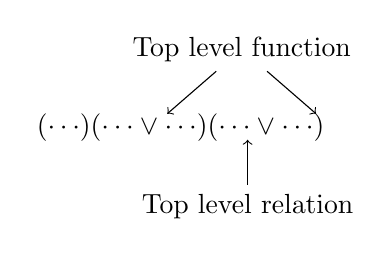
\begin{tikzpicture}
    \node (text) at (0,0) {$\always{(\cdots)} \proves (\cdots \lor \cdots) \wand (\cdots \lor \cdots)$};
    \node (rel) at (.85,-1) {Top level relation};
    \draw[->] (rel) -- (.85,-.15);
    \node (func) at (.775,1) {Top level function};
    \draw[->] (func) -- (-.17, .18);
    \draw[->] (func) -- (1.72, .18);
  \end{tikzpicture}
\end{center}
Using these descriptions we show a proof using our monotone proof search. Then, we outline the steps we took in this proof.
\begin{example}{$\isMLL_\hopred$\ is monotone}{ismllproper}
  The predicate $\isMLL_\hopred$ is monotone in its first argument. Thus, $\isMLL_\hopred$ is a proper element of
  \[
    \persrel (\point \point \wandrel) \respect \point \point \wandrel
  \]
  In other words
  \[
    \always{(\All \hd\, \vect{v}. \pred\, \hd\, \vect{v} \wand \predB\, \hd\, \vect{v})} \wand \All \hd\, \vect{v}. \isMLL_\hopred\, \pred\, \hd\, \vect{v} \wand \isMLL_\hopred\, \predB\, \hd\, \vect{v}
  \]


  \begin{proof}
    We assume any premises, $\always{(\All \hd\, \vect{v}. \pred\, \hd\, \vect{v} \wand \predB\, \hd\, \vect{v})}$. We omit the premises in future proof states, but it is always there since it is persistent. Next, we introduce the universal quantifiers. After unfolding $\isMLL_\hopred$, we have to prove the following.
    \begin{align*}
      (\cdots \lor \cdots \pred \cdots) \wand (\cdots \lor \cdots \predB \cdots)
    \end{align*}
    Thus, the top level connective is the wand and the one below it is the disjunction. We now search for a signature ending on a magic wand and which has the disjunction as a proper element. We find the signature ${\wandrel \respect \wandrel \respect \wandrel}$ with $\lorrel$. We apply $(\wandrel \respect \wandrel \respect \wandrel) \lorrel \lorrel$ resulting in two statements to prove.
    \begin{align*}
       & (\hd = \None * \vect{\val} = []) \wand (\hd = \None * \vect{\val} = [])                                \\
       & (\cdots \pred \cdots \lor \cdots  \pred \cdots) \wand (\cdots \predB \cdots \lor \cdots \predB \cdots)
    \end{align*}
    The first statement follows directly from reflexivity of the magic wand. The second statement utilizes the same disjunction signature again, thus we just show the end results of applying it.
    \begin{align*}
       & (\Exists \loc, \val', \tl. \cdots \pred \cdots) \wand (\Exists \loc, \val', \tl. \cdots \predB \cdots)                               \\
       & (\Exists \loc, \val', \vect{\val}'', \tl. \cdots \pred \cdots) \wand (\Exists \loc, \val', \vect{\val}'', \tl. \cdots \predB \cdots)
    \end{align*}
    Both statements have as top level relation $\wandrel$ with below it $\exists$. We apply the signature of $\exists$ with as result.
    \begin{align*}
       & \All \loc. (\Exists \val', \tl. \cdots \pred \cdots) \wand (\Exists \val', \tl. \cdots \predB \cdots)                               \\
       & \All \loc. (\Exists \val', \vect{\val}'', \tl. \cdots \pred \cdots) \wand (\Exists \val', \vect{\val}'', \tl. \cdots \predB \cdots)
    \end{align*}
    We introduce $\loc$ and repeat these steps until the existential quantification is no longer the top level function.
    \begin{align*}
       & (\hd = \Some l * l \fmapsto (\val', \True, \tl) * \pred\, \tl\, \vect{\val}) \wand \\
       & (\hd = \Some l * l \fmapsto (\val', \True, \tl) * \predB\, \tl\, \vect{\val})      \\
       &
      \left(\begin{array}{@{}l}
                \hd = \Some l * l \fmapsto (\val', \False, \tl)\spac * \\
                \vect{\val} = \val' :: \vect{\val}'' * \pred\, \tl\, \vect{\val}''
              \end{array}\right)
      \wand                                                                                 \\
       & \left(\begin{array}{@{}l}
                   \hd = \Some l * l \fmapsto (\val', \False, \tl)\spac * \\
                   \vect{\val} = \val' :: \vect{\val}'' * \predB\, \tl\, \vect{\val}''
                 \end{array}\right)
    \end{align*}
    We can now repeatedly apply the signature of $\seprel$ and apply reflexivity for any created propositions without $\pred$ or $\predB$. This leaves us with
    \begin{align*}
      \always{(\All \hd\, \vect{v}. \pred\, \hd\, \vect{v} \wand \predB\, \hd\, \vect{v})} & \proves \pred\, \tl\, \vect{\val} \wand \predB\, \tl\, \vect{\val}     \\
      \always{(\All \hd\, \vect{v}. \pred\, \hd\, \vect{v} \wand \predB\, \hd\, \vect{v})} & \proves \pred\, \tl\, \vect{\val}'' \wand \predB\, \tl\, \vect{\val}''
    \end{align*}
    These hold from the assumption.
  \end{proof}
\end{example}
The strategy we use for proof search consists of two steps. We have a normalization step, and we have an application step.
\begin{description}
  \item[Normalization] Introduce any universal quantifiers, extra created wands and modalities. Afterwards, do an application step.
  \item[Application] We apply the first option that works.
        \begin{enumerate}
          \item If left and right-hand side of the relation are equal, and the relation is reflexive, apply reflexivity.
          \item Check if the conclusion follows from a premise, and then apply it.
          \item Look for a signature of the top level function where the last relation matches the top level relation of the conclusion. Apply it if we find one. Next, do a normalization step.
        \end{enumerate}
\end{description}
We start the proof with the normalization step and continue until all created branches are proven.

\paragraph{Generating the fixpoints theorem}
Given the above proof of monotonicity of $\isMLL_\hopred$, \cref{thm:leastfixpoint} does not give a least fixpoint for $\isMLL_\hopred$. We change the definition to add an arbitrary amount of arguments to the fixpoint and its properties.
\[
  \lfp\hopred\,\var_1\,\cdots\,\var_n \eqdef \All \pred. \always(\All \varB_1,\cdots,\varB_n. \hopred\, \pred\, \varB_1\,\cdots\,\varB_n \wand \pred\, \varB_1\,\cdots\,\varB_n) \wand \pred \, \var_1\,\cdots\,\var_n
\]
This is not a valid definition in our logic for an arbitrary $n$. Thus, we create a least fixpoint theorem for any function we want to take a fixpoint of.
\begin{example}{$\isMLL$ least fixpoint theorem}{ismlllfp}
  We have the monotone function
  \[ \isMLL_\hopred\colon (\Val \to \List\ \Val \to \iProp) \to \Val \to \List\ \Val \to \iProp \]
  We use the above definition of the least fixpoint with $n = 2$.
  \[ \lfp\isMLL_\hopred\,\hd\,\vect{\val} \eqdef \All \pred. \always(\All \hd',\vect{\val}'. \isMLL_\hopred\, \pred\, \hd'\, \vect{\val}' \wand \pred\, \hd'\, \vect{\val}') \wand \pred\, \hd\, \vect{\val} \]
\end{example}
For the induction principle we apply the same strategy. For $\isMLL$ we get the induction principle as described in \cref{ex:irisisMLL}.

\end{document}
